\documentclass[a4paper,12pt,twoside]{memoir}

% Castellano
\usepackage[spanish,es-tabla]{babel}
\selectlanguage{spanish}
\usepackage[utf8]{inputenc}
\usepackage[T1]{fontenc}
\usepackage{lmodern} % scalable font
\usepackage{microtype}
\usepackage{placeins}
\usepackage{lscape}

\RequirePackage{booktabs}
\RequirePackage[table]{xcolor}
\RequirePackage{xtab}
\RequirePackage{multirow}

% Links
\PassOptionsToPackage{hyphens}{url}\usepackage[colorlinks]{hyperref}
\hypersetup{
	allcolors = {red}
}

% Ecuaciones
\usepackage{amsmath}

% Rutas de fichero / paquete
\newcommand{\ruta}[1]{{\sffamily #1}}

% Párrafos
\nonzeroparskip

% Huérfanas y viudas
\widowpenalty100000
\clubpenalty100000

% Evitar solapes en el header
\nouppercaseheads

% Imagenes
\usepackage{graphicx}
\newcommand{\imagen}[2]{
	\begin{figure}[!h]
		\centering
		\includegraphics[width=0.9\textwidth]{#1}
		\caption{#2}\label{fig:#1}
	\end{figure}
	\FloatBarrier
}

\usepackage{graphicx}
\newcommand{\imagenentidad}[2]{
	\begin{figure}[!h]
		\centering
		\includegraphics[width=0.5\textwidth]{#1}
		\caption{#2}\label{fig:#1}
	\end{figure}
	\FloatBarrier
}

\usepackage{graphicx}
\newcommand{\imagenapaisada}[2]{
	\begin{figure}[!h]
		\centering
		\includegraphics[width=1.4\textwidth]{#1}
		\caption{#2}\label{fig:#1}
	\end{figure}
	\FloatBarrier
}

\usepackage{graphicx}
\newcommand{\imagensprint}[2]{
	\begin{figure}[!h]
		\centering
		\includegraphics[width=0.8\textwidth]{#1}
		\caption{#2}\label{fig:#1}
	\end{figure}
	\FloatBarrier
}

\newcommand{\imagenflotante}[2]{
	\begin{figure}%[!h]
		\centering
		\includegraphics[width=0.9\textwidth]{#1}
		\caption{#2}\label{fig:#1}
	\end{figure}
}



% El comando \figura nos permite insertar figuras comodamente, y utilizando
% siempre el mismo formato. Los parametros son:
% 1 -> Porcentaje del ancho de página que ocupará la figura (de 0 a 1)
% 2 --> Fichero de la imagen
% 3 --> Texto a pie de imagen
% 4 --> Etiqueta (label) para referencias
% 5 --> Opciones que queramos pasarle al \includegraphics
% 6 --> Opciones de posicionamiento a pasarle a \begin{figure}
\newcommand{\figuraConPosicion}[6]{%
  \setlength{\anchoFloat}{#1\textwidth}%
  \addtolength{\anchoFloat}{-4\fboxsep}%
  \setlength{\anchoFigura}{\anchoFloat}%
  \begin{figure}[#6]
    \begin{center}%
      \Ovalbox{%
        \begin{minipage}{\anchoFloat}%
          \begin{center}%
            \includegraphics[width=\anchoFigura,#5]{#2}%
            \caption{#3}%
            \label{#4}%
          \end{center}%
        \end{minipage}
      }%
    \end{center}%
  \end{figure}%
}

%
% Comando para incluir imágenes en formato apaisado (sin marco).
\newcommand{\figuraApaisadaSinMarco}[5]{%
  \begin{figure}%
    \begin{center}%
    \includegraphics[angle=90,height=#1\textheight,#5]{#2}%
    \caption{#3}%
    \label{#4}%
    \end{center}%
  \end{figure}%
}
% Para las tablas
\newcommand{\otoprule}{\midrule [\heavyrulewidth]}
%
% Nuevo comando para tablas pequeñas (menos de una página).
\newcommand{\tablaSmall}[5]{%
 \begin{table}
  \begin{center}
   \rowcolors {2}{gray!35}{}
   \begin{tabular}{#2}
    \toprule
    #4
    \otoprule
    #5
    \bottomrule
   \end{tabular}
   \caption{#1}
   \label{tabla:#3}
  \end{center}
 \end{table}
}

%
%Para el float H de tablaSmallSinColores
\usepackage{float}

%
% Nuevo comando para tablas pequeñas (menos de una página).
\newcommand{\tablaSmallSinColores}[5]{%
 \begin{table}[H]
  \begin{center}
   \begin{tabular}{#2}
    \toprule
    #4
    \otoprule
    #5
    \bottomrule
   \end{tabular}
   \caption{#1}
   \label{tabla:#3}
  \end{center}
 \end{table}
}

\newcommand{\tablaApaisadaSmall}[5]{%
\begin{landscape}
  \begin{table}
   \begin{center}
    \rowcolors {2}{gray!35}{}
    \begin{tabular}{#2}
     \toprule
     #4
     \otoprule
     #5
     \bottomrule
    \end{tabular}
    \caption{#1}
    \label{tabla:#3}
   \end{center}
  \end{table}
\end{landscape}
}

%
% Nuevo comando para tablas grandes con cabecera y filas alternas coloreadas en gris.
\newcommand{\tabla}[6]{%
  \begin{center}
    \tablefirsthead{
      \toprule
      #5
      \otoprule
    }
    \tablehead{
      \multicolumn{#3}{l}{\small\sl continúa desde la página anterior}\\
      \toprule
      #5
      \otoprule
    }
    \tabletail{
      \hline
      \multicolumn{#3}{r}{\small\sl continúa en la página siguiente}\\
    }
    \tablelasttail{
      \hline
    }
    \bottomcaption{#1}
    \rowcolors {2}{gray!35}{}
    \begin{xtabular}{#2}
      #6
      \bottomrule
    \end{xtabular}
    \label{tabla:#4}
  \end{center}
}

%
% Nuevo comando para tablas grandes con cabecera.
\newcommand{\tablaSinColores}[6]{%
  \begin{center}
    \tablefirsthead{
      \toprule
      #5
      \otoprule
    }
    \tablehead{
      \multicolumn{#3}{l}{\small\sl continúa desde la página anterior}\\
      \toprule
      #5
      \otoprule
    }
    \tabletail{
      \hline
      \multicolumn{#3}{r}{\small\sl continúa en la página siguiente}\\
    }
    \tablelasttail{
      \hline
    }
    \bottomcaption{#1}
    \begin{xtabular}{#2}
      #6
      \bottomrule
    \end{xtabular}
    \label{tabla:#4}
  \end{center}
}

%
% Nuevo comando para tablas grandes sin cabecera.
\newcommand{\tablaSinCabecera}[5]{%
  \begin{center}
    \tablefirsthead{
      \toprule
    }
    \tablehead{
      \multicolumn{#3}{l}{\small\sl continúa desde la página anterior}\\
      \hline
    }
    \tabletail{
      \hline
      \multicolumn{#3}{r}{\small\sl continúa en la página siguiente}\\
    }
    \tablelasttail{
      \hline
    }
    \bottomcaption{#1}
  \begin{xtabular}{#2}
    #5
   \bottomrule
  \end{xtabular}
  \label{tabla:#4}
  \end{center}
}



\definecolor{cgoLight}{HTML}{EEEEEE}
\definecolor{cgoExtralight}{HTML}{FFFFFF}

%
% Nuevo comando para tablas grandes sin cabecera.
\newcommand{\tablaSinCabeceraConBandas}[5]{%
  \begin{center}
    \tablefirsthead{
      \toprule
    }
    \tablehead{
      \multicolumn{#3}{l}{\small\sl continúa desde la página anterior}\\
      \hline
    }
    \tabletail{
      \hline
      \multicolumn{#3}{r}{\small\sl continúa en la página siguiente}\\
    }
    \tablelasttail{
      \hline
    }
    \bottomcaption{#1}
    \rowcolors[]{1}{cgoExtralight}{cgoLight}

  \begin{xtabular}{#2}
    #5
   \bottomrule
  \end{xtabular}
  \label{tabla:#4}
  \end{center}
}




\graphicspath{ {./img/} }

% Capítulos
\chapterstyle{bianchi}
\newcommand{\capitulo}[2]{
	\setcounter{chapter}{#1}
	\setcounter{section}{0}
	\setcounter{figure}{0}
	\setcounter{table}{0}
	\chapter*{#2}
	\addcontentsline{toc}{chapter}{#2}
	\markboth{#2}{#2}
}

% Apéndices
\renewcommand{\appendixname}{Apéndice}
\renewcommand*\cftappendixname{\appendixname}

\newcommand{\apendice}[1]{
	%\renewcommand{\thechapter}{A}
	\chapter{#1}
}

\renewcommand*\cftappendixname{\appendixname\ }

% Formato de portada
\makeatletter
\usepackage{xcolor}
\newcommand{\tutor}[1]{\def\@tutor{#1}}
\newcommand{\course}[1]{\def\@course{#1}}
\definecolor{cpardoBox}{HTML}{E6E6FF}
\def\maketitle{
  \null
  \thispagestyle{empty}
  % Cabecera ----------------
\noindent
\includegraphics[width=\textwidth]{cabecera}\vspace{1cm}%
  \vfill
  % Título proyecto y escudo informática ----------------
  \colorbox{cpardoBox}{%
    \begin{minipage}{.8\textwidth}
      \vspace{.5cm}\Large
      \begin{center}
      \textbf{TFG del Grado en Ingeniería Informática}\vspace{.6cm}\\
      \textbf{\LARGE\@title{}}
      \end{center}
      \vspace{.2cm}
    \end{minipage}

  }%
  \hfill\begin{minipage}{.20\textwidth}
    
\includegraphics[width=\textwidth]{escudoInfor}
  \end{minipage}
  \vfill
  % Datos de alumno, curso y tutores ------------------
  \begin{center}%
  {%
    \noindent\LARGE
    Presentado por \@author{}\\ 
    en Universidad de Burgos --- \@date{}\\
    Tutores: \@tutor{}\\
  }%
  \end{center}%
  \null
  \cleardoublepage
  }
\makeatother


% Datos de portada
\title{{\Huge DeltaOffers}\\[0.5cm] Portal de convocatorias de PDI Y PAS de las Universidades de Castilla y León}
\author{Miguel Ubierna Gutiérrez}
\tutor{Dr. César Ignacio Garcia Osorio\\y Dra. Ana Serrano Mamolar}
\date{\today}

\begin{document}

\maketitle



\cleardoublepage



%%%%%%%%%%%%%%%%%%%%%%%%%%%%%%%%%%%%%%%%%%%%%%%%%%%%%%%%%%%%%%%%%%%%%%%%%%%%%%%%%%%%%%%%



\frontmatter


\clearpage

% Indices
\tableofcontents

\clearpage

\listoffigures

\clearpage

\listoftables

\clearpage

\mainmatter

\appendix

\apendice{Plan de Proyecto Software}

\section{Introducción}
En los años actuales, se viene dando gran prioridad a dedicar tiempo y recursos para realizar una  planificación del proyecto de calidad. Esto se debe a que en todo proyecto es muy importante asentar unas bases sólidas de planificación y de estructura antes de ponernos a trabajar en los aspectos más técnicos.

Este plan de proyecto nos indicará los pasos a seguir para que el resultado de un proyecto sea satisfactorio y por lo tanto se consiga alcanzar el éxito.

Esta fase de planificación va a estar fragmentada en dos partes:
\begin{itemize}
\item 
\textbf{Planificación temporal: } Donde se detallarán los plazos que se han seguido en el proyecto y las distintas tareas y actividades realizadas en estos mismos.
\item 
\textbf{Estudio de viabilidad: } Donde se realizará un estudio económico con su respectivo análisis de costes y beneficios y, por otro lado, un estudio legal en el que se analizarán todas las leyes que pueden llegar a estar involucradas en el proyecto.
\end{itemize}

Ambas partes deben de tenerse en cuenta a la hora de realizar un proyecto y si se realizan correctamente, estaremos en una situación ventajosa para llevar a cabo el proyecto con el menor número de contratiempos y problemas posibles. 
\section{Planificación temporal}
La gestión de este proyecto se ha llevado a cabo siguiendo una metodología Scrum~\cite{scrum:latex}, metodología basada en \textit{sprints}. Durante estos \textit{sprints} de dos semanas de duración, se acordaba una reunión retrospectiva con los tutores en la cual se hacían revisiones de las tareas realizadas durante el \textit{sprint} y se planteaban nuevas tareas para \textit{sprints} futuros.

Todas estas tareas abordadas, han sido recogidas dentro del apartado \textit{Issues} en la plataforma de desarrollo colaborativo con control de versiones basado en Git (Github). Además, durante estos \textit{spints}, también se iban subiendo a esta misma plataforma, los distintos desarrollos realizados.

Por otro lado, cabe destacar que la metodología ágil Scrum no se ha podido realizar en su totalidad dado que es una metodología diseñada para grupos de trabajo y este proyecto ha sido un proyecto individual.

Finalmente, se van a detallar cuáles han sido los \textit{sprints} realizados con algunas descripciones de las tareas y actividades realizadas. Además, se mostrarán una serie de gráficas con el porcentaje de tiempo dedicado en el sprint a las distintas actividades realizadas.

\subsection{Sprint 1 (08/02/2024 -
21/02/2024)}

Este \textit{sprint} comenzó con una reunión inicial con mis tutores César Ignacio García Osorio y Ana Serrano Mamolar tras haber acordado su mentorización para este proyecto previamente. En esta reunión se determinaron los objetivos del proyecto realizando una estructuración de este.

Por otro lado, también se trató el tema de las herramientas que iban a ser utilizadas para la realización del proyecto, buscando unas herramientas que se adaptasen a las tareas que se iban a realizar y al objetivo final que se quería conseguir. 

Finalmente, se me dieron algunos consejos en función de las dudas que tenía sobre como estructurar y organizar el proyecto en cuanto a tiempos y a las actividades a realizar.


El trabajo realizado estas dos semanas consistió en:
\begin{itemize}
\item 
\textbf{Investigación de las webs de las que voy a extraer información mediante \textit{web scraping}: } Para determinar todos los atributos candidatos a recopilar para mostrarlos en la web de mi proyecto.
\item 
\textbf{Determinar las bibliotecas de Python que van a ser utilizadas para llevar a cabo el proceso de \textit{web scraping} }

\end{itemize}

\imagensprint{sprint1}{Sprint 1.}

\subsection{Sprint 2 (22/02/2024 -
06/03/2024)}
Durante esta segunda iteración se realizó el proceso de \textit{web scraping} para las universidades públicas de Castilla y León. Esta fue una primera toma de contacto con el \textit{scraping} en la que se obtuvieron los atributos de cada una de las convocatorias y para cada una de las universidades.

Para este proceso se utilizaron herramientas como Requests ~\cite{requests:latex}, Selenium ~\cite{selenium:latex} y BeautifulSoup ~\cite{beautifulsoup:latex}. Durante este \textit{sprint} se fue aprendiendo la utilización de estas herramientas mediante la lectura de documentación y su aplicación práctica.

Además, dado que la calidad de algunos datos cuando se realizó el \textit{scraping} no eran buenos, se decidió realizar la limpieza de algunos de ellos ya pensando en la calidad de mi web en el futuro.

Por último, se realizó una subida al repositorio del proyecto en GitHub con los desarrollos realizados durante este \textit{sprint}.

\imagensprint{sprint2}{Sprint 2.}

\subsection{Sprint 3 (07/03/2024 -
20/03/2024)}
Por un lado, este periodo consistió en añadir funcionalidad nueva al proceso de \textit{web scraping} mediante la explotación de nuevos atributos los cuales no habían sido contemplados anteriormente.

Sin embargo, también se buscó mucho mejorar la calidad del código realizado hasta esta fecha. Para ello se decidió pasar el desarrollo realizado a programación orientada a objetos teniendo así una estructura mucho más definida y favoreciendo de esta manera la eliminación de duplicidad de código. De esta manera, se estructuró el proyecto con una clase por cada una de las universidades de las que se extrajeron los datos.

Por último, se aplicó la guía de estilos de \textit{PEP8}  para mejorar la legibilidad y calidad del código. Esto se hizo con una herramienta disponible para Python llamada Autopep8~\cite{autopep8:latex} la cual nos aplicaba la guía de estilos al guardar los cambios en el desarrollo realizado.

\imagensprint{sprint3}{Sprint 3.}

\subsection{Sprint 4 (21/03/2024 -
03/04/2024)}
En esta iteración, se realizó una limpieza de los datos recopilados en cuanto a su formato y se comenzó a utilizar herencia mediante la creación de una clase abstracta con los métodos comunes de las clases concretas. Este aspecto mejora enormemente la extensibilidad y facilidad de mantenimiento del código para situaciones futuras.

Gran parte del tiempo del sprint, se dedicó a la implantación de \textit{testing}. Esto se debe a que los test unitarios en los proyectos de desarrollo de software tienen un valor crucial en la detección de errores y mejora de mantenimiento. Además, aseguran que el software tenga una cierta calidad. Para este proceso se utilizaron herramientas como MagicMock y UnitTest ~\cite{unittest:latex}.

Por otro lado, se creó un entorno virtual en Python con \textit{virtualenv} para la gestión de dependencias y de esta manera aislar el entorno en el que se está desarrollando el proyecto ~\cite{virtualenv:latex}.

Finalmente, se creó un directorio en el proyecto con un fichero en el que se realizaban las llamadas a las correspondientes clases en las que se desarrolló el \textit{web scraping} de cada una de las universidades para recopilar la información. Todos estos datos fueron recopilados y se realizó una conexión con la base de datos para que fuesen almacenados ahí de forma segura.

\imagensprint{sprint4}{Sprint 4.}

\subsection{Sprint 5 (04/04/2024 -
17/04/2024)}
Los primeros días de este periodo, consistieron en corregir algunos errores que se percibieron al ejecutar los test de aspectos que no se estaban realizando del todo bien en el proceso de \textit{web scraping}. Una vez ya realizada esta tarea, se realizaron las inserciones de los datos recopilados con un formato adecuado a una base de datos MySQL ~\cite{mysqlpython:latex}. Esta base de datos puede ser considerado un almacén de datos o \textit{Data Warehouse} en el que aparecían los atributos comunes y no comunes entre las distintas webs de las distintas universidades junto con una recopilación de todas las convocatorias.

Una vez realizado esto, se comenzó con el desarrollo de la web que iba a recoger todas estas convocatorias del PDI y PAS. Para realizar esta web se decidió optar por un \textit{framework} como Asp .NET Core MVC el cual es utilizado para realizar aplicaciones web siguiendo el patrón Modelo-Vista-Controlador ~\cite{aspnetcore:latex}.

Por otro lado, también se realizaron algunas tareas de \textit{mockup} pensando en diseños atractivos para la aplicación web a realizar. En el momento que se encontraron una serie de prototipos acordes con la idea principal, se comenzó a trabajar con HTML y CSS para la realización de las interfaces.

Finalmente, se utilizaron \textit{media queries} para que la web tuviera un diseño \textit{responsive}  y, de esta manera, que se pudiese utilizar en cualquier tipo de pantalla sin importar las dimensiones de esta.

\imagensprint{sprint5}{Sprint 5.}

\subsection{Sprint 6 (18/04/2024 -
01/05/2024)}

Durante este \textit{sprint}, se realizaron con diseño adaptativo las ventanas en las que aparecen los detalles de cada una de las convocatorias.

Posteriormente, para añadir funcionalidad extra a mi aplicación web, se decidió integrar el inicio de sesión con Google mediante autenticación basada en OAuth 2.0 ~\cite{autenticaciongoogle:latex}. Esto se realizó para que se pudiese permitir la integración con Google Calendar desde la web y de esta manera aportar un valor extra a la aplicación.

La integración con Google Calendar también se realizó en este sprint ~\cite{googlecalendar:latex}. De esta manera, los usuarios que iniciasen sesión con la aplicación podrán añadir a su calendario la fecha en la que caduca esa convocatoria y así poder acordarse de realizar solicitudes en el caso de que estén interesados.

Con la finalización de este \textit{sprint} se consideraba que la funcionalidad de la aplicación se había acabado de desarrollar en su totalidad.

\imagensprint{sprint6}{Sprint 6.}

\subsection{Sprint 7 (02/05/2024 -
15/05/2024)}
Esta iteración, fue una de las finales del proyecto y como consecuencia, se dedicó gran parte del tiempo para realizar la documentación. Para ello, se recopilaron todas las anotaciones, datos y tareas de los anteriores \textit{sprints}. 

Por otro lado, se ha comenzado a dedicar gran parte del tiempo a la investigación sobre las distintas posibilidades que hay para lanzar la aplicación de manera gratuita para que pueda ser probada por cualquier usuario.

Por último, dado que la integración con Google Calendar solo era viable realizarla con usuarios de \textit{testing}, se decidió eliminar esta integración e incorporar a la web un sistema de avisos por correo en la que se enviaban adjuntos archivos ICalendar para que cada usuario pudiese añadir sus convocatorias de interés como eventos a sus calendarios personales ~\cite{icalendar:latex}.

En este sprint, al igual que en la mayoría de los anteriores, también se dedicó parte de tiempo a corrección de errores y mejoras.
\imagensprint{sprint7}{Sprint 7.}


\subsection{Sprint 8 (16/05/2024 -
30/05/2024)}
En esta etapa, se continuó trabajando con la documentación del proyecto. Además, pese a tener algunos problemas con algunas herramientas utilizadas para hacer el \textit{deployment}, se acabó realizando satisfactoriamente mediante la utilización de un plan gratuito de Azure Services ~\cite{azureservices:latex}. 

Por otro lado, se realizó la implementación de un \textit{cron} para mantener la base de datos actualizada. Esto lo pude hacer gracias a GitHub Actions ~\cite{githubactions:latex}.

Finalmente, también se realizó alguna mejora en el código. Hasta ahora, para la importación de paquetes se estaba trabajando con rutas relativas y para un mejor despliegue, se comenzaron a utilizar rutas absolutas. Este es uno de los cambios más destacables en cuanto a código en esta iteración.
\imagensprint{sprint8}{Sprint 8.}

\subsection{Sprint 9 (31/05/2024 -
12/06/2024)}
Con esta iteración se pondría broche final al proyecto. Ya con el despliegue de la aplicación realizado, se dedicó la mayoría del tiempo a la preparación de la documentación y últimos detalles del proyecto para entregarlo al tribunal.

Se realizaron las últimas mejoras en el código,  y se realizó una carga del proyecto en una máquina virtual. Esta máquina virtual se almacenará en un USB para su posterior entrega al tribunal.

\imagensprint{sprint9}{Sprint 9.}

\subsection{Resumen}

Una vez finalizados todos los \textit{sprints} se han podido obtener una serie de conclusiones sobre cómo ha sido la planificación del proyecto y el tiempo que se ha invertido en cada una de las distintas actividades y tareas, estas conclusiones se van a comentar a continuación:

\begin{itemize}
\item En las primeras iteraciones, como es lógico, se invirtió gran parte del tiempo a la planificación y estructuración del proyecto.

\item En casi todos los \textit{sprints} se ha dedicado un porcentaje de tiempo a la programación y a la realización de nuevos desarrollos.

\item El soporte y las mejoras de la aplicación, fue algo frecuente en gran parte de las iteraciones gracias a la implementación de \textit{testing} y realización de test manuales mediante el uso de la aplicación, se pudieron corregir los errores.

\item Una vez que acabaron los desarrollos en cuanto a la extracción de datos, se dedicó más tiempo al prototipado y al desarrollo de las interfaces de la aplicación.

\item Los últimos tramos del proyecto fueron dedicados a la documentación de la aplicación y a su lanzamiento.

\end{itemize}

\section{Estudio de viabilidad}

\subsection{Viabilidad económica}

\subsubsection{Introducción}
En este apartado se va a realizar un análisis de los costes y los beneficios que tendría este proyecto. Estos factores serán muy importantes en el caso de que este proyecto se ejecutase en un entorno real. De esta manera podríamos examinar su viabilidad financiera e incluso apreciar cual sería el impacto que tienen los costes y beneficios a la hora de tomar decisiones.

Por otro lado, dado que el proyecto no se ha llevado a cabo  en un entorno real, podría haber otros factores que afecten a la viabilidad económica del mismo y que no hayan sido detallados en este apartado.

\subsubsection{Análisis de los Costes}

En este apartado, podemos identificar tres categorías de costes que casi todo proyecto software se encuentra en el camino:  los costes humanos, los costes de hardware y los costes de software.

\textbf{Costes humanos:}

Este proyecto ha sido realizado por una sola persona. Considerando que ese empleado es un Ingeniero Informático cuyo país de residencia es España, según el portal \textit{Talent.com} al que puedes acceder desde el siguiente \href{https://es.talent.com/salary?job=ingeniero+inform%C3%A1tico}{enlace}, el salario promedio por hora es de 13,86 € ~\cite{salarioingeniero:latex}. Contando que se han dedicado 300 horas, podemos deducir lo siguiente:

\[ 13,86 \, \text{€} \times 300 \, \text{horas} = 4158 \, \text{€ brutos totales} \]

Esta cantidad la tenemos que dividir entre los 4 meses en los que se ha realizado en proyecto y por lo tanto:

\[ 4158 \, \text{€} / 4 \, \text{meses} = 1039,5 \, \text{€ brutos mensuales} \]

Una vez analizado lo que va a recibir el trabajador, vamos a analizar cuáles serían, como consecuencia, los costes totales de personal que tendrá la empresa ~\cite{costetrabajador:latex}:
 

\begin{table}[H]
    \centering
    \renewcommand{\arraystretch}{1.2}
    \setlength{\tabcolsep}{20pt}
    \begin{tabular}{l l}
        \hline
        \textbf{Concepto} & \textbf{Coste} \\ \hline
        Salario mensual bruto & 1039,5€ \\
        Contingencias comunes (23,6\%) & 245,32€\\
        Tipo general de  desempleo (5,5\%) & 57,17€\\
        Contingencias profesionales (3,5\%) & 36,38€\\
        Fondo de garantía social (0,2\%)& 2,08€\\
        Formación profesional (0,6\%) & 6,24€\\
        Salario mensual total & 1386,69€\\  \hline
        \textbf{Total costes humanos} & \textbf{5546,76€}\\ \hline
    \end{tabular}
    \caption{Costes humanos totales}
    \label{tab:costes_humanos}
\end{table}

\newpage

\textbf{Costes hardware:}

Para el desarrollo del proyecto, tan solo es necesario poseer de un ordenador portátil. En este caso, suponemos que el ordenador ha sido comprado nuevo por la empresa para la realización de este nuevo proyecto. Contando con que el proceso de \textit{web scraping} es costoso en cuanto a rendimiento, se necesitará un ordenador con unas características medianamente potentes, por lo tanto, el coste hardware será el siguiente:

\begin{table}[H]
    \centering
    \renewcommand{\arraystretch}{1.2}
    \setlength{\tabcolsep}{20pt}
    \begin{tabular}{l l}
        \hline
        \textbf{Concepto} & \textbf{Coste} \\ \hline
        Ordenador Portátil & 879,99€ \\  \hline
        \textbf{Total costes hardware} & \textbf{879,99€}\\ \hline
    \end{tabular}
    \caption{Costes hardware}
    \label{tab:costes_hardware}
\end{table}

\textbf{Costes software:}

En cuanto a los costes software, tan solo podríamos recalcar el sistema operativo utilizado, pero en este caso, la licencia venía con el ordenador portátil de fábrica. Este sistema operativo era el Windows 10 Pro.

Por otro lado, me gustaría destacar que todas las herramientas software utilizadas son gratuitas. Esto es un factor muy a tener en cuenta a la hora de realizar un estudio económico del proyecto dado que reduce enormemente los costes en comparación con otros proyectos.

\textbf{Otros costes:}
Aunque este tipo de costes no estén encasillados en una categoría como las definidas previamente. Un proyecto de este estilo suele necesitar de otros productos o servicios que también son imprescindibles para que el proyecto tenga éxito.  

Los productos y servicios mencionados previamente se consideran los siguientes:

\begin{itemize}
\item \textbf{Infraestructura de alojamiento y dominio: } Dado que para este tipo de proyectos es necesario disponer de instancias de computación en la nube y un dominio personalizado.
\item \textbf{Conexión a internet: } Debido a que a pesar de que el software sea gratuito, se necesita en ocasiones conexión con la red para poder ejecutarlo.
\item \textbf{Documentación impresa y material para la presentación: } Dado que es necesario por si se quieren tener reuniones con posibles compradores del producto o para presentarlo dentro de la empresa en la que se ha realizado el proyecto. En este caso esto se ha realizado para poder presentarlo ante el tribunal.

\end{itemize}

\begin{table}[H]
    \centering
    \setlength{\tabcolsep}{20pt}
    \begin{tabular}{l l}
        \hline
        \textbf{Concepto} & \textbf{Coste} \\ \hline
        Infraestructura y Dominio & 65,55€ \\
        Internet  & 87,60€\\
        Documentación y material para la presentación & 50€\\  \hline
        \textbf{Total otros costes} & \textbf{203,15€}\\ \hline
    \end{tabular}
    \caption{Otros Costes}
    \label{tab:otros_costes}
\end{table}


\textbf{Costes totales:}

Una vez analizados todos los costes anteriores, podemos calcular cuales han sido los costes totales:

\begin{table}[H]
    \centering
    \renewcommand{\arraystretch}{1.2}
    \setlength{\tabcolsep}{20pt}
    \begin{tabular}{l l}
        \hline
        \textbf{Concepto} & \textbf{Coste} \\ \hline
        Costes Humanos & 5546,76€ \\
        Costes Software & 0€ \\
        Costes Hardware  & 879,99€\\
        Otros costes & 203,15€\\  \hline
        \textbf{Costes Totales} & \textbf{6629,9€}\\ \hline
    \end{tabular}
    \caption{Costes Totales}
    \label{tab:costes_totales}
\end{table}

\textbf{Beneficios:}

El objetivo de esta aplicación ha sido aportar un servicio a las universidades de Castilla y León mediante una aplicación en la que se pudiesen ver recopiladas todas las convocatorias que estas universidades publican en sus webs. 

Por esta razón, en caso de que la aplicación pasase a desarrollo, esta misma se distribuirá de manera gratuita para un beneficio de la comunidad universitaria.

Por otro lado, si se quisiese obtener un beneficio económico de la misma, se podría plantear la implantación de anuncios y publicidad. Otra opción válida como modelo de negocio, sería el cobro de un importe para aquellos usuarios que hayan accedido a una convocatoria gracias a esta web y hayan sido elegidos para el puesto solicitado.

\subsection{Viabilidad legal}
Al igual que la viabilidad económica, la viabilidad legal también es un aspecto muy importante para considerar a la hora de planificar un proyecto software. Este apartado va a consistir en el análisis del cumplimiento de leyes por parte del proyecto y las licencias de software. 

En primer lugar, en cuanto al contenido multimedia utilizado, ha sido obtenido en distintas webs cuyos contenidos están libres de \textit{copyright} bajo la licencia \textbf{CC0 (Creative Commons Zero)} ~\cite{codigoabierto:latex}. Esto implica que ese contenido multimedia puede ser utilizado sin tener permisos debido a que no están protegidas por derechos de autor. En este caso, se ha dado alguna excepción a la hora de obtener los logos de las distintas universidades involucradas en el proyecto.

Estas imágenes han sido obtenidas a través de las webs de las propias universidades. En principio, dado que esto es un proyecto educativo, estas imágenes pueden ser utilizadas sin ningún inconveniente. Además, en el caso de que el proyecto pasase a desarrollo, no se prevé tener ningún inconveniente en este aspecto legal con las mismas dado que los beneficiarios de que esta aplicación pasase a desarrollo serían las propias universidades.

Posteriormente, se van a analizar las licencias de las dependencias utilizadas en el proyecto. Este proceso lo vamos a dividir en 2 partes. En primer lugar se van a analizar las dependencias utilizadas en cuanto al proceso de \textit{web scraping} realizado con Python. Estas dependencias se han aparecerán listadas en el fichero \textit{requirements.txt} del proyecto y serán las siguientes:

\begin{table}[H]
    \centering
    \renewcommand{\arraystretch}{1.2} % Ajusta el espacio entre filas
    \begin{tabularx}{\textwidth}{l l X l}
        \hline
        \textbf{Dependencia} & \textbf{Versión} & \textbf{Descripción} & \textbf{Licencia} \\
        \hline
        autopep8 & 2.0.4 & Guía de estilos para Python & MIT \\
        beautifulsoup4 & 4.12.3 & Biblioteca para la extracción de datos en HTML & MIT \\
        mysql-connector-python & 8.3.0 & Herramienta para conexión con la base de datos & GPL \\
        pillow & 10.3.0 & Biblioteca para el tratamiento de imágenes & BSD \\
        pytest & 8.1.1 & Herramienta para implementación de testing & MIT \\
        requests & 2.31.0 & Biblioteca para hacer peticiones HTTP & Apache2 \\
        selenium & 4.18.1 & Herramienta automatización sitio web & Apache2 \\
        \hline
    \end{tabularx}
    \caption{Dependencias junto con sus Licencias Python}
    \label{tab:licencias1}
\end{table}

\newpage
Posteriormente, veremos los paquetes que han sido instalados en .NET para la realización de la web junto con sus respectivas licencias:

\begin{table}[H]
    \centering
    \renewcommand{\arraystretch}{1.2} % Ajusta el espacio entre filas
    \begin{tabularx}{\textwidth}{X l X l}
        \hline
        \textbf{Dependencia} & \textbf{Versión} & \textbf{Descripción} & \textbf{Licencia} \\
        \hline
        X PagedList Mvc Core & 9.1.2 & Herramienta para aplicar paginación & MIT \\
        Pomelo Entity Framework Core MySql& 8.0.2 & Herramienta para la conexión con la base de datos & MIT \\
        MySql Entity Framework Core & 8.0.2 & Herramienta para conexión con la base de datos & MIT \\
        Microsoft
        Entity Framework Core & 8.0.3 & Herramienta para acceso a bases de datos & Apache2 \\
        Microsoft Entity Framework Core Tools & 8.0.3 & Herramienta para el trabajo con bases de datos mediante objetos & Apache2 \\
        Mailkit & 4.6.0 & Herramienta envío de emails & Apache2 \\
        \hline
    \end{tabularx}
    \caption{Dependencias junto con sus Licencias .NET}
    \label{tab:licencias2}
\end{table}

Tal y como hemos podido apreciar anteriormente, la mayoría de las dependencias de este proyecto tienen una licencia de software MIT o Apache v2.0 ambas licencias son bastante permisivas y disponen de gran disponibilidad en cuanto a su uso.

Una vez evaluado lo anterior, se ha decidido que el código fuente sea público para que pueda ser modificado, estudiado y utilizado por cualquier persona sin restricciones de propiedad intelectual o de licencia. Por lo tanto, la licencia otorgada al proyecto será una licencia \textbf{MIT} esta licencia permite a los usuarios utilizar, modificar y distribuir el software sin restricciones, siempre y cuando se proporcione atribución al autor original y se incluya un aviso de derechos de autor en todas las copias del software ~\cite{licenciamit:latex}.

Además, otro aspecto importante a considerar es que esta licencia nos permite compatibilidad con Apache v2.0. Algo que puede ser ventajoso de cara al futuro y nuevas implementaciones.

Mediante la elección de esta licencia se contribuye enormemente con la comunidad dado que el producto se podrá utilizar y compartir con total libertad.



\apendice{Especificación de Requisitos}

\section{Introducción}

La especificación de requisitos en un proyecto software consiste en describir cómo se va a comportar el sistema que ha sido desarrollado. En este apartado, se detallarán los distintos casos de uso los cuales describen las distintas acciones o actividades que va a realizar un actor para que finalmente se lleve a cabo algún proceso ~\cite{especificacionrequisitos:latex}.

Tanto los requisitos como los casos de uso son muy importantes en este tipo de proyectos dado que se detallan las funciones que va a realizar el sistema de manera concisa. Además, esto mejora enormemente la comunicación entre el equipo que ha desarrollado el software y el cliente o usuarios finales. Por último, la especificación de estos requisitos cuando se inicia un proyecto ayuda a localizar los posibles inconvenientes con los que se puede encontrar el equipo de desarrollo a lo largo del mismo.

\section{Objetivos generales}

En este apartado se van a comentar cuales han sido los objetivos del proyecto, algunos de ellos fueron propuestos en las fases iniciales del proyecto, sin embargo, muchos otros se han añadido después para mejorar la funcionalidad de la aplicación web y que esta sea más completa y de mejor calidad. Los objetivos en su totalidad han sido los siguientes:

\begin{itemize}

\item Recopilación de convocatorias de Personal Docente Investigador y Personal de Administración y Servicios de las Universidades públicas de Castilla y León de sus respectivas páginas web. 

\item Interpretar los datos obtenidos, tratamiento de estos y almacenarlos de manera segura.

\item Proporcionar a las personas interesadas en este tipo de ofertas, una web unificada que listase todas estas convocatorias con un formato unificado. Además, esta web mejorará en usabilidad y en funcionalidad a las webs en las que las universidades publican sus convocatorias.

\item Proporcionar el acceso a información más detallada de estas convocatorias junto con un enlace que te redirige a la web original.

\item Permitir que las personas puedan recibir correos con un archivo adjunto para que puedan añadir las convocatorias a sus respectivos calendarios.

\end{itemize}

\section{Catálogo de requisitos}

Una vez mencionados los objetivos, se enumerarán los requisitos funcionales y no funcionales del proyecto:

\textbf{Requisitos funcionales:}

\begin{itemize}
\item\textbf{RF-1 Recopilación de datos}: La aplicación tiene que ser capaz de recopilar datos de las distintas webs mediante \textit{web scraping}.
\begin{itemize}
\item\textbf{RF-1.1 Tratamiento de datos}: La aplicación debe ser capaz de tratar los datos e interpretarlos.
\begin{itemize}
\item\textbf{RF-1.1.1 Estructuración de datos}: La aplicación debe estructurar los datos obtenidos para que estos tengan un formato y estructura uniforme.
\end{itemize}
\item\textbf{RF-1.2 Almacenamiento de datos}: La aplicación debe almacenar los datos recopilados de forma segura en una base de datos.
\item\textbf{RF-1.3 Actualización de los datos}: Los datos mostrados en la aplicación deben de ser actualizados periódicamente con las últimas actualizaciones en las webs de origen.
\end{itemize}
\end{itemize}

\begin{itemize}
\item\textbf{RF-2 Visualización de las convocatorias}: La aplicación tiene que ser capaz de mostrar la información de las distintas convocatorias.
\begin{itemize}
\item\textbf{RF-2.1 Mostrar listado maestro de las convocatorias}: La aplicación debe de listar en una página \textit{maestra} la información esencial y descriptiva de cada convocatoria, esto se realizará de manera paginada.
\item\textbf{RF-2.2 Aplicación de filtros}: La web tiene que permitir la aplicación de filtros para que los usuarios puedan acceder más rápido a las convocatorias de interés.
\item\textbf{RF-2.3 Mostrar Detalles}: La aplicación debe de tener páginas \textit{detalle} con los detalles de las convocatorias que el usuario selecciona.

\end{itemize}

\item\textbf{RF-3 Acceso al portal de convocatorias de las universidades}: La aplicación tiene que permitir al usuario acceder mediante un enlace en la página de detalles a las páginas webs propias de cada universidad.

\item\textbf{RF-4 Activar avisos}: El usuario debe poder activar avisos en las convocatorias que le interesen.

\begin{itemize}
\item\textbf{RF-4.1 Suscripción a avisos por correo}: El usuario debe poder suscribirse a recibir avisos por medio del correo electrónico.
\begin{itemize}
\item\textbf{RF-4.1.1 Comprobación correo válido}: La aplicación debe comprobar si el correo con el que el usuario se ha suscrito es válido.
\end{itemize}
\item\textbf{RF-4.2 Recibir avisos}: La aplicación debe enviar avisos por correo de las convocatorias que el usuario desea y el usuario deberá recibir estos.
\item\textbf{RF-4.3 Recibir archivos ICalendar adjuntos}: La aplicación debe generar un archivo ICalendar con la fecha fin de las convocatorias y adjuntarlo en el correo enviado al usuario.
\begin{itemize}
\item\textbf{RF-4.3.1 Compatibilidad ICalendar con principales servicios de calendario}: La aplicación debe proporcionar un archivo de extensión \textit{".ics"} que debe de ser compatible con Outlook, Google Calendar y otros.
\end{itemize}
\item\textbf{RF-4.4 Acceso al portal de convocatorias de las universidades}: En el correo electrónico que recibe el usuario se debe permitir acceder mediante un enlace en la página de detalles a las páginas webs propias de cada universidad.
\end{itemize}
\item\textbf{RF-5 Comienzo de uso de la web}: La aplicación debe mostrar una ventana principal con información de la temática de la web junto con un acceso para comenzar su uso.
\end{itemize}

\textbf{Requisitos no funcionales:}

\begin{itemize}
\item\textbf{RNF-1 Rendimiento:} Los tiempos de respuesta son aceptables contando que se está utilizando un servidor web gratuito. La aplicación siempre responde ante las peticiones correctamente, aunque el tiempo de respuesta en ocasiones no sea inmediato.
\item\textbf{RNF-2 Seguridad:} Los
datos obtenidos serán almacenados de manera segura sin que se pueda acceder de manera no autorizada. 
\item\textbf{RNF-3 Usabilidad:} La experiencia del usuario al interactuar con el sistema es buena. La web es intuitiva y fácil de utilizar. La curva de aprendizaje es muy pequeña. 
\item\textbf{RNF-4 Disponibilidad:} La aplicación web está disponible para los usuarios siempre y cuando tengan conexión a internet.
\item\textbf{RNF-5 Mantenibilidad:} La aplicación web será fácil de mantener siempre y cuando la estructura HTML de las webs de las que se extraen los datos sea la misma. En el caso de que no, la web necesitará de soporte. La implementación de test unitarios facilita enormemente este aspecto.
\item\textbf{RNF-6 Escalabilidad:} La estructura del proyecto está diseñada para que la aplicación sea fácilmente escalable gracias a la aplicación de buenas prácticas y patrones de diseño.
\item\textbf{RNF-7 Portabilidad:} La página web puede ser accedida desde cualquier navegador. Además, tiene un diseño adaptativo para que sea compatible con multitud de dispositivos independientemente del ancho de la pantalla.

\end{itemize}

\section{Especificación de requisitos}
En este apartado se mostrará un diagrama de los casos de uso basándonos en los requisitos previamente mencionados. Posteriormente, se detallarán cada uno de estos.

\newpage
\begin{landscape}
\subsection{Diagrama de casos de uso}\label{diagrama-de-casos-de-uso}
\vspace{1cm}
\imagenapaisada{DiagramaCasosUsoTFG}{Diagrama de casos de uso.}
\end{landscape}
\newpage

\subsection{Actores}
Los actores en un diagrama de casos de uso, son aquellos que desempeñan alguna función dentro del sistema. Los actores no tienen por qué ser una sola persona sino también un equipo o un sistema externo. En el caso de nuestro sistema, hemos encontrado gran diversidad en cuanto a los actores:

\begin{itemize}
\item\textbf{Usuario}: Son aquellos que van a utilizar la aplicación y dispondrán de toda la funcionalidad de esta. La aplicación está diseñada para que el usuario pueda interactuar con ella de una manera sencilla y con una buena experiencia de usuario.
\item\textbf{Equipo desarrollo/soporte}: En este proyecto, los desarrolladores y el equipo de soporte, también realizan acciones que impactan en el sistema. Esto se debe a que, dado que nuestra web está constantemente recopilando datos de webs externas, en el caso de que nuevas convocatorias de nuevas universidades se quieran mostrar en la web o que cambie la estructura de la actual web de origen, el equipo de desarrollo y soporte tendrán que realizar labores de tratamiento de datos, estructuración y almacenamiento.
\item\textbf{Sistema cron}: Este sistema ha sido el encargado de actualizar la base de datos periódicamente según se iban actualizando las convocatorias en las webs de las propias universidades. De esta manera, la información en la web del proyecto, estaba actualizada constantemente.
\item\textbf{Sistema de correo}: Por último, otro de los actores involucrados ha sido el sistema de correo. Este ha permitido el envío de avisos a los usuarios que van a utilizar la web. En este caso, el sistema utilizado ha sido el servidor de correo electrónico SMTP, el cual permite el envío de emails de manera automatizada.
\end{itemize}


\begin{table}[p]
	\centering
	\begin{tabularx}{\linewidth}{ p{0.21\columnwidth} p{0.71\columnwidth} }
		\toprule
		\textbf{CU-1}    & \textbf{Recopilación de datos}\\
		\toprule
		\textbf{Versión}              & 1.0    \\
		\textbf{Autor}                & Miguel Ubierna Gutiérrez \\
		\textbf{Requisitos asociados} & RF-1, RF-1.1, RF-1.1.1, RF-1.2, RF-1.3,  \\
		\textbf{Descripción}          & La aplicación deberá disponer de las convocatorias que las universidades muestran en sus propias webs. \\
		\textbf{Precondición}         & Las webs de las correspondientes universidades deberán estar disponibles. \\
		\textbf{Acciones}             &
		\begin{enumerate}
			\def\labelenumi{\arabic{enumi}.}
			\tightlist
			\item El equipo de desarrollo examinará la estructura de las webs para su extracción de datos.
			\item Recopilará los datos más interesantes.
                \item Se tratarán los datos recopilados y se almacenarán los mismos.
                \item Los datos se mostrarán de manera actualizada en la web mediante el sistema \textit{cron}.
		\end{enumerate}\\
		\textbf{Postcondición}        & La base de datos será actualizada. \\
		\textbf{Excepciones}          & Fallo en las solicitudes HTTP a las correspondientes webs. \\
		\textbf{Importancia}          & Alta. \\
		\bottomrule
	\end{tabularx}
	\caption{CU-1 Recopilación de datos.}
\end{table}


\begin{table}[p]
	\centering
	\begin{tabularx}{\linewidth}{ p{0.21\columnwidth} p{0.71\columnwidth} }
		\toprule
		\textbf{CU-2}    & \textbf{Tratamiento de datos}\\
		\toprule
		\textbf{Versión}              & 1.0    \\
		\textbf{Autor}                & Miguel Ubierna Gutiérrez \\
		\textbf{Requisitos asociados} & RF-1.1, RF-1.1.1 \\
		\textbf{Descripción}          & La aplicación debe ser capaz de tratar los datos, para que solo sean mostrados aquellos que sean descriptivos y de interés. \\
		\textbf{Precondición}         & Que se hayan podido recopilar los datos correctamente. \\
		\textbf{Acciones}             &
		\begin{enumerate}
			\def\labelenumi{\arabic{enumi}.}
			\tightlist
			\item Se obtienen todos los datos.
			\item Se detectan los datos no válidos o erróneos
                \item Se detectan los datos que no son de interés.
                \item Se trabaja con los datos de interés
		\end{enumerate}\\
		\textbf{Postcondición}        & Ninguna. \\
		\textbf{Excepciones}          & Ninguna. \\
		\textbf{Importancia}          & Alta.  \\
		\bottomrule
	\end{tabularx}
	\caption{CU-2 Tratamiento de datos.}
\end{table}


\begin{table}[p]
	\centering
	\begin{tabularx}{\linewidth}{ p{0.21\columnwidth} p{0.71\columnwidth} }
		\toprule
		\textbf{CU-3}    & \textbf{Estructuración de datos}\\
		\toprule
		\textbf{Versión}              & 1.0    \\
		\textbf{Autor}                & Miguel Ubierna Gutiérrez \\
		\textbf{Requisitos asociados} & RF-1.1.1 \\
		\textbf{Descripción}          & La aplicación debe ser capaz de tratar los datos, para que después estos sean mostrados con una estructura y formato correctos. \\
		\textbf{Precondición}         & Se debe disponer de los datos de interés. \\
		\textbf{Acciones}             &
		\begin{enumerate}
			\def\labelenumi{\arabic{enumi}.}
			\tightlist
			\item Se obtienen los datos de interés.
			\item Se estructuran los mismos por categorías o importancia.
                \item Se corrigen las divergencias en cuanto a los formatos.
                \item Se almacenan los mismos de manera correcta.
		\end{enumerate}\\
		\textbf{Postcondición}        & La base de datos debe estar disponible. \\
		\textbf{Excepciones}          & Ninguna.  \\
		\textbf{Importancia}          & Media.  \\
		\bottomrule
	\end{tabularx}
	\caption{CU-3 Estructuración de datos.}
\end{table}

\begin{table}[p]
	\centering
	\begin{tabularx}{\linewidth}{ p{0.21\columnwidth} p{0.71\columnwidth} }
		\toprule
		\textbf{CU-4}    & \textbf{Almacenamiento de datos}\\
		\toprule
		\textbf{Versión}              & 1.0    \\
		\textbf{Autor}                & Miguel Ubierna Gutiérrez \\
		\textbf{Requisitos asociados} & RF-1.2 \\
		\textbf{Descripción}          & La aplicación debe ser capaz de almacenar los datos de interés que ya tienen el formato adecuado. \\
		\textbf{Precondición}         & Disponer de una base de datos.\\
		\textbf{Acciones}             &
		\begin{enumerate}
			\def\labelenumi{\arabic{enumi}.}
			\tightlist
			\item Se configura un servidor para almacenar la base de datos.
			\item Se crean las bases de datos en el servidor.
                \item La aplicación se conecta con el servidor para transferir sus datos al mismo.
                \item Se almacenan los datos de manera correcta.
		\end{enumerate}\\
		\textbf{Postcondición}        & El servidor debe estar disponible. \\
		\textbf{Excepciones}          & El servidor no está disponible, no se cargarán las convocatorias.  \\
		\textbf{Importancia}          & Alta.  \\
		\bottomrule
	\end{tabularx}
	\caption{CU-4 Almacenamiento de datos.}
\end{table}

\begin{table}[p]
	\centering
	\begin{tabularx}{\linewidth}{ p{0.21\columnwidth} p{0.71\columnwidth} }
		\toprule
		\textbf{CU-5}    & \textbf{Actualización de los datos}\\
		\toprule
		\textbf{Versión}              & 1.0    \\
		\textbf{Autor}                & Miguel Ubierna Gutiérrez \\
		\textbf{Requisitos asociados} & RF-1.3 \\
		\textbf{Descripción}          & La aplicación debe ser capaz de mostrar las ofertas de manera actualizada basándose en las webs sobre las que se extraen los datos. \\
		\textbf{Precondición}         & Disponer conexión con el servidor de base de datos.\\
		\textbf{Acciones}             &
		\begin{enumerate}
			\def\labelenumi{\arabic{enumi}.}
			\tightlist
			\item Se configura un sistema \textit{cron} para que los datos se actualicen de manera periódica.
			\item El sistema \textit{cron} ejecuta determinados \textit{scripts} de la aplicación para que la web este actualizada.
                \item Se almacenan los datos actualizados en la base de datos.
		\end{enumerate}\\
		\textbf{Postcondición}        & Las ofertas estarán actualizadas. \\
		\textbf{Excepciones}          & El servidor no está disponible, no se cargarán las nuevas convocatorias.  \\
		\textbf{Importancia}          & Alta.  \\
		\bottomrule
	\end{tabularx}
	\caption{CU-5 Actualización de los datos.}
\end{table}


\begin{table}[p]
	\centering
	\begin{tabularx}{\linewidth}{ p{0.21\columnwidth} p{0.71\columnwidth} }
		\toprule
		\textbf{CU-6}    & \textbf{Visualización de las convocatorias}\\
		\toprule
		\textbf{Versión}              & 1.0    \\
		\textbf{Autor}                & Miguel Ubierna Gutiérrez \\
		\textbf{Requisitos asociados} & RF-2, RF-2.1, RF-2.2, RF-2.3, \\
		\textbf{Descripción}          & Permite que el usuario pueda visualizar las convocatorias recopiladas de las distintas webs de las universidades.  \\
		\textbf{Precondición}         & Disponer conexión con el servidor de base de datos.\\
		\textbf{Acciones}             &
		\begin{enumerate}
			\def\labelenumi{\arabic{enumi}.}
			\tightlist
   			\item Se cargan las respectivas convocatorias de las bases de datos.
			\item El usuario empieza con el uso de la aplicación.
			\item El usuario podrá ver las convocatorias.
		\end{enumerate}\\
		\textbf{Postcondición}        & Ninguna. \\
		\textbf{Excepciones}          & El servidor que aloja la base de datos no está disponible, no se cargarán las convocatorias.  \\
		\textbf{Importancia}          & Alta.  \\
		\bottomrule
	\end{tabularx}
	\caption{CU-6 Visualización de las convocatorias.}
\end{table}


\begin{table}[p]
	\centering
	\begin{tabularx}{\linewidth}{ p{0.21\columnwidth} p{0.71\columnwidth} }
		\toprule
		\textbf{CU-7}    & \textbf{Mostrar listado maestro de las convocatorias}\\
		\toprule
		\textbf{Versión}              & 1.0    \\
		\textbf{Autor}                & Miguel Ubierna Gutiérrez \\
		\textbf{Requisitos asociados} & RF-2.1 \\
		\textbf{Descripción}          & Permite al usuario visualizar un listado maestro de las convocatorias con los atributos más descriptivos de las mismas.  \\
		\textbf{Precondición}         & Disponer  de conexión con el servidor de base de datos.\\
		\textbf{Acciones}             &
		\begin{enumerate}
			\def\labelenumi{\arabic{enumi}.}
			\tightlist
			\item El usuario accede a la página maestra de la aplicación.
                \item Se cargan las respectivas convocatorias de las bases de datos.
			\item Se mostrará un listado paginado de las convocatorias con los atributos más descriptivos de las mismas como la categoría, plazo y universidad.
		\end{enumerate}\\
		\textbf{Postcondición}        & Ninguna. \\
		\textbf{Excepciones}          & El servidor que aloja la base de datos no está disponible, no se cargarán las convocatorias.  \\
		\textbf{Importancia}          & Alta.  \\
		\bottomrule
	\end{tabularx}
	\caption{CU-7 Mostrar listado maestro de las convocatorias.}
\end{table}


\begin{table}[p]
	\centering
	\begin{tabularx}{\linewidth}{ p{0.21\columnwidth} p{0.71\columnwidth} }
		\toprule
		\textbf{CU-8}    & \textbf{Aplicación de filtros}\\
		\toprule
		\textbf{Versión}              & 1.0    \\
		\textbf{Autor}                & Miguel Ubierna Gutiérrez \\
		\textbf{Requisitos asociados} & RF-2.2 \\
		\textbf{Descripción}          & Permite al usuario aplicar los filtros que este desea para que encuentre de manera rápida las convocatorias de su interés.  \\
		\textbf{Precondición}         & Las convocatorias deben de cargar correctamente.\\
		\textbf{Acciones}             &
		\begin{enumerate}
			\def\labelenumi{\arabic{enumi}.}
			\tightlist
			\item Se mostrará un listado paginado de las convocatorias con los atributos más descriptivos de las mismas como la categoría, plazo y universidad.
                \item El usuario podrá filtrar por estos campos.
                \item Una vez se pulse el botón 'Filtrar' se aplicarán los filtros.
                \item Se mostrarán las convocatorias filtradas y paginadas.
		\end{enumerate}\\
		\textbf{Postcondición}        & Las convocatorias devueltas deben de ser solo las que cumplen el filtro. \\
		\textbf{Excepciones}          & Ninguna.  \\
		\textbf{Importancia}          & Media.  \\
		\bottomrule
	\end{tabularx}
	\caption{CU-8 Aplicación de filtros.}
\end{table}


\begin{table}[p]
	\centering
	\begin{tabularx}{\linewidth}{ p{0.21\columnwidth} p{0.71\columnwidth} }
		\toprule
		\textbf{CU-9}    & \textbf{Mostrar detalles}\\
		\toprule
		\textbf{Versión}              & 1.0    \\
		\textbf{Autor}                & Miguel Ubierna Gutiérrez \\
		\textbf{Requisitos asociados} & RF-2.3 \\
		\textbf{Descripción}          & Permite al usuario ver detalles de las convocatorias por las que está interesado con información adicional a la que se mostraba en el listado maestro.  \\
		\textbf{Precondición}         & Las convocatorias deben de cargar correctamente.\\
		\textbf{Acciones}             &
		\begin{enumerate}
			\def\labelenumi{\arabic{enumi}.}
			\tightlist
			\item El usuario detecta en el listado una convocatoria que es de su interés.
                \item Accede a los detalles de la misma.
                \item Se mostrará información más detallada de la convocatoria junto con los atributos mostrados en el listado.
		\end{enumerate}\\
		\textbf{Postcondición}        & Se deberán mostrar los detalles de la convocatoria que ha seleccionado el usuario. \\
		\textbf{Excepciones}          & Ninguna  \\
		\textbf{Importancia}          & Media  \\
		\bottomrule
	\end{tabularx}
	\caption{CU-9 Mostrar detalles.}
\end{table}

\begin{table}[p]
	\centering
	\begin{tabularx}{\linewidth}{ p{0.21\columnwidth} p{0.71\columnwidth} }
		\toprule
		\textbf{CU-10}    & \textbf{Acceso al portal de convocatorias de las universidades}\\
		\toprule
		\textbf{Versión}              & 1.0    \\
		\textbf{Autor}                & Miguel Ubierna Gutiérrez \\
		\textbf{Requisitos asociados} & RF-3, RF-4.4 \\
		\textbf{Descripción}          & Permite a los usuarios acceder mediante un enlace a las secciones de las webs donde las propias universidades suben sus convocatorias.  \\
		\textbf{Precondición}         & Los detalles de las convocatorias deben haber cargado correctamente.\\
		\textbf{Acciones}             &
		\begin{enumerate}
			\def\labelenumi{\arabic{enumi}.}
			\tightlist
			\item El usuario accede a los detalles de una convocatoria desde el listado general.
                \item Dentro de la ventana detalles habrá un enlace que redirigirá al usuario a la propia web de la universidad correspondiente.
                \item El usuario visualizará la convocatoria correspondiente y podrá ofrecerse como candidato realizando los trámites requeridos por la universidad.
                \item El usuario también podrá acceder desde el correo cuando realiza una suscripción para recibir avisos.                
		\end{enumerate}\\
		\textbf{Postcondición}        & Ninguna \\
		\textbf{Excepciones}          & Ninguna  \\
		\textbf{Importancia}          & Alta  \\
		\bottomrule
	\end{tabularx}
	\caption{CU-10 Acceso al portal de convocatorias de las universidades.}
\end{table}


\begin{table}[p]
	\centering
	\begin{tabularx}{\linewidth}{ p{0.21\columnwidth} p{0.71\columnwidth} }
		\toprule
		\textbf{CU-11}    & \textbf{Activar Avisos}\\
		\toprule
		\textbf{Versión}              & 1.0    \\
		\textbf{Autor}                & Miguel Ubierna Gutiérrez \\
		\textbf{Requisitos asociados} & RF-4, RF-4.1, RF-4.1.1, RF-4.2, RF-4.3, RF-4.3.1, RF-4.4  \\
		\textbf{Descripción}          & Permite que el sistema de correo pueda enviar avisos sobre las convocatorias a los usuarios.  \\
		\textbf{Precondición}         & El listado de las convocatorias ha debido de cargar correctamente.\\
		\textbf{Acciones}             &
		\begin{enumerate}
			\def\labelenumi{\arabic{enumi}.}
			\tightlist
			\item El usuario visualiza el listado maestro de las convocatorias.
                \item Selecciona la opción de obtener avisos en la convocatoria en la que está interesado.
                \item Si la validación es correcta, se enviará el aviso correspondiente.
		\end{enumerate}\\
		\textbf{Postcondición}        & El email debe ser enviado al correo electrónico proporcionado. \\
		\textbf{Excepciones}          & Ventana de error en el caso de que el correo no sea correcto.  \\
		\textbf{Importancia}          & Baja.  \\
		\bottomrule
	\end{tabularx}
	\caption{CU-11 Activar Avisos.}
\end{table}


\begin{table}[p]
	\centering
	\begin{tabularx}{\linewidth}{ p{0.21\columnwidth} p{0.71\columnwidth} }
		\toprule
		\textbf{CU-12}    & \textbf{Suscripción a avisos por correo}\\
		\toprule
		\textbf{Versión}              & 1.0    \\
		\textbf{Autor}                & Miguel Ubierna Gutiérrez \\
		\textbf{Requisitos asociados} & RF-4.1, RF-4.1.1  \\
		\textbf{Descripción}          & Permite que el usuario se suscriba al sistema de avisos de la \textit{app} para recibir avisos de las convocatorias que el desee.  \\
		\textbf{Precondición}         & Ninguna.\\
		\textbf{Acciones}             &
		\begin{enumerate}
			\def\labelenumi{\arabic{enumi}.}
			\tightlist
			\item El usuario indica que quiere recibir avisos de una determinada convocatoria.
                \item El usuario deberá rellenar un formulario con su email y aceptar recibir emails.
                \item Una vez realizado esto, el usuario ya estará suscrito para recibir avisos.
		\end{enumerate}\\
		\textbf{Postcondición}        & Ninguna. \\
		\textbf{Excepciones}          & Ventana error en el caso de suscripción incorrecta.  \\
		\textbf{Importancia}          & Baja.  \\
		\bottomrule
	\end{tabularx}
	\caption{CU-12 Suscripción a avisos por correo.}
\end{table}


\begin{table}[p]
	\centering
	\begin{tabularx}{\linewidth}{ p{0.21\columnwidth} p{0.71\columnwidth} }
		\toprule
		\textbf{CU-13}    & \textbf{Comprobación correo valido}\\
		\toprule
		\textbf{Versión}              & 1.0    \\
		\textbf{Autor}                & Miguel Ubierna Gutiérrez \\
		\textbf{Requisitos asociados} & RF-4.1.1  \\
		\textbf{Descripción}          & La aplicación dispone de un sistema de validación de correos para asegurarse de que el usuario completa correctamente el formulario.  \\
		\textbf{Precondición}         & Ninguna.\\
		\textbf{Acciones}             &
		\begin{enumerate}
			\def\labelenumi{\arabic{enumi}.}
			\tightlist
			\item El usuario acepta la recepción de emails para ser avisado de una determinada convocatoria.
                \item Si el email es válido, se enviará el aviso.
                \item Se mostrará una alerta en la que indica que el aviso ha sido enviado correctamente.
		\end{enumerate}\\
		\textbf{Postcondición}        & Ninguna. \\
		\textbf{Excepciones}          & Ventana error en el caso de que el correo no sea válido. \\
		\textbf{Importancia}          & Baja.  \\
		\bottomrule
	\end{tabularx}
	\caption{CU-13 Comprobación correo valido.}
\end{table}


\begin{table}[p]
	\centering
	\begin{tabularx}{\linewidth}{ p{0.21\columnwidth} p{0.71\columnwidth} }
		\toprule
		\textbf{CU-14}    & \textbf{Recibir archivos ICalendar adjuntos}\\
		\toprule
		\textbf{Versión}              & 1.0    \\
		\textbf{Autor}                & Miguel Ubierna Gutiérrez \\
		\textbf{Requisitos asociados} & RF-4.3  \\
		\textbf{Descripción}          & El sistema de correo enviará archivos ICalendar adjuntos con la fecha de fin de las convocatorias para que los usuarios puedan añadirlo a sus calendarios personales.  \\
		\textbf{Precondición}         & Ninguna.\\
		\textbf{Acciones}             &
		\begin{enumerate}
			\def\labelenumi{\arabic{enumi}.}
			\tightlist
			\item El usuario se suscribe a los avisos correctamente.
                \item El usuario recibe un email con el aviso y el archivo ICalendar.
                \item El archivo ICalendar puede ser abierto por el usuario y añadirlo a su calendario personal.
		\end{enumerate}\\
		\textbf{Postcondición}        & Deberá aparecer un nuevo evento en el calendario personal del usuario. \\
		\textbf{Excepciones}          & Ninguna. \\
		\textbf{Importancia}          & Baja.  \\
		\bottomrule
	\end{tabularx}
	\caption{CU-14 Recibir archivos ICalendar adjuntos.}
\end{table}


\begin{table}[p]
	\centering
	\begin{tabularx}{\linewidth}{ p{0.21\columnwidth} p{0.71\columnwidth} }
		\toprule
		\textbf{CU-15}    & \textbf{Compatibilidad ICalendar}\\
		\toprule
		\textbf{Versión}              & 1.0    \\
		\textbf{Autor}                & Miguel Ubierna Gutiérrez \\
		\textbf{Requisitos asociados} & RF-4.3.1  \\
		\textbf{Descripción}          & El archivo de extension \textit{.ics} deberá ser compatible con los principales servicios de calendario.\\
		\textbf{Precondición}         & El archivo ICalendar se ha debido de generar correctamente.\\
		\textbf{Acciones}             &
		\begin{enumerate}
			\def\labelenumi{\arabic{enumi}.}
			\tightlist
                \item El usuario abre el archivo con su correo.
                \item El evento se añadirá a los servicios de calendario más populares como Google Calendar o Outlook.
		\end{enumerate}\\
		\textbf{Postcondición}        & Deberá aparecer un nuevo evento en el calendario personal del usuario. \\
		\textbf{Excepciones}          & Si el formato no es compatible, le aparecerá una excepción al usuario. \\
		\textbf{Importancia}          & Baja.  \\
		\bottomrule
	\end{tabularx}
	\caption{CU-15 Compatibilidad ICalendar.}
\end{table}



\apendice{Especificación de diseño}

\section{Introducción}

En esta apartado, se van a constatar las especificaciones de diseño de este proyecto. Estas especificaciones de diseño van acorde a los objetivos propuestos al principio del proyecto y a los requisitos funcionales y no funcionales mencionados previamente. El diseño del sistema, lo podemos dividir en tres partes:

\begin{itemize}
    \item \textbf{Diseño de datos:} Define como se estructuran y almacenan los datos del sistema. Este proceso es muy importante para entender cómo se relacionan los datos y cómo definir una estructura ventajosa para el programa y sus correspondientes procedimientos.
    \item \textbf{Diseño de procedimental:} Indica los algoritmos y procedimientos utilizados en el sistema. En este proceso, suelen utilizarse los diagramas de flujo como representación gráfica de los algoritmos utilizados. 
    \item \textbf{Diseño arquitectónico:} Que el sistema posea de una buena arquitectura, es enormemente ventajoso para que sea robusto y eficiente. En este apartado se especificará cual es la arquitectura del sistema y sus principales componentes. Además, se explicarán los patrones de diseño aplicados en el proyecto.
\end{itemize}

\section{Diseño de datos}

Esta aplicación tan solo cuenta con dos entidades, las cuales son 'Convocatorias' y 'Suscripciones'. Se tomó esa decisión dado que con tan solo la creación de dos entidades se podías satisfacer los objetivos que tenía la aplicación.

Los atributos e información de interés de las correspondientes convocatorias se pueden encapsular en una sola tabla sin necesidad de relaciones con otras entidades lo cual podría suponer una pérdida de eficiencia cuando se acceden a los datos. A continuación, se va a mostrar la entidad junto con los atributos que tiene.

\imagenentidad{EntidadTFG}{Entidad Convocatorias.}

Por otro lado, para evitar que la aplicación se utilizase como herramienta se span, se limitó el número de avisos que se podían recibir por correo mensualmente. Para gestionar esto, se generó otra tabla con los emails registrados y el número de avisos que se habían enviado a ese determinado email. A continuación, se muestra gráficamente la entidad.

\imagenentidad{EntidadSuscripciones}{Entidad Suscripciones.}

\section{Diseño procedimental}

En este apartado se van a detallar los procedimientos que va a realizar un usuario al utilizar la aplicación. Para ello, se va a realizar un diagrama de flujo para indicar de manera esquematizada los distintos procedimientos y flujos que el usuario puede seguir al utilizar la aplicación. 

\newpage
\begin{landscape}
\subsection{Diagrama de flujo}
\imagenapaisada{DiagramaDeFlujo}{Diagrama de flujo.}
\end{landscape}
\newpage

\section{Diseño arquitectónico}
La arquitectura software es la encargada de diseñar la estructura que va a tener el sistema. Tener una arquitectura consistente es fundamental en aspectos de eficiencia, mantenibilidad y seguridad.

En esta fase de estructuración del sistema, juegan un papel muy importante los patrones de diseño los cuales proporcionan una mayor eficiencia y calidad de software.
Además, la utilización de estos patrones mejora la escalabilidad de los proyectos permitiendo que estos puedan crecer pero continuando con una estructura sólida.

En este apartado, se va a comentar la arquitectura general del sistema y los patrones de diseño que han sido utilizados a lo largo del proyecto. Algunos de estos patrones han sido aplicados a la parte de web scraping mientras que otros han sido aplicados a la hora de realizar la web. Todos los patrones utilizados, se comentarán a continuación.

\subsection{Patrones de diseño y arquitectura}

\subsubsection{Patrón de Arquitectura MVC (Modelo-Vista-Controlador)}
Este patrón \cite{patronmvc:latex} se utiliza para que la interfaz de usuario, los datos y la lógica de la aplicación, trabajen de manera desacoplada. Con este patrón utilizado para aplicaciones web, las solicitudes se enrutan a un controlador que es el que trabaja con el modelo de datos y, finalmente, elige la vista que se va a mostrar pasándole el modelo de datos. Más detalladamente, las capas de este patrón consisten en lo siguiente:

\begin{itemize}
    \item \textbf{Modelo:} en esta capa se encontrará una representación de los datos del dominio y la lógica de negocio de la aplicación con las que podemos gestionar entidades. El modelo es el que nos proporciona los datos que utilizamos en la aplicación y nos permite almacenarlos correctamente.
    \item \textbf{Vista:} La vista es la que se encarga de que se visualicen las interfaces de nuestra aplicación. En la vista se podrán visualizar los datos del modelo que la vista ha recibido a través del controlador.
    Para esta parte de la vista, se han utilizado las \textit{Razor Pages} dado que nos permiten incluir lógica en C\# dentro del HTML.
    \item \textbf{Controlador:} Este actúa como intermediario entre el usuario y el sistema. Este es el encargado de enviar información desde el modelo a la vista y viceversa.
\end{itemize}

\begin{figure}[H]
    \centering
    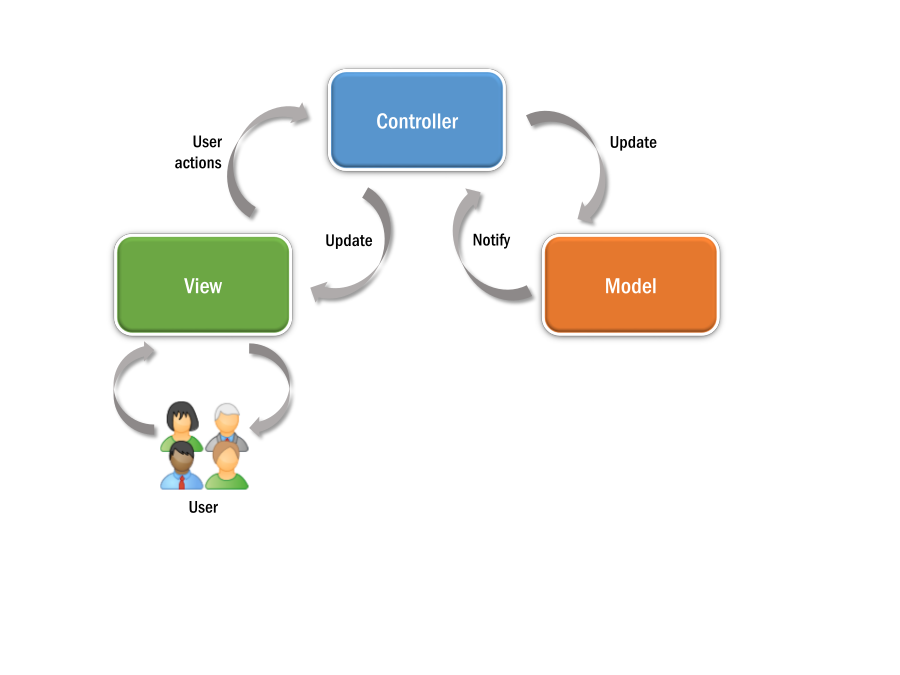
\includegraphics[width=0.9\linewidth]{DocumentacionTFG//img/PatronMVC.png}
    \caption{Patrón Modelo-Vista-Controlador}
\end{figure}

\subsubsection{Patrón Inyección de dependencias}

Este es un patrón de diseño admitido por .NET en el que las dependencias de una determinada clase, no necesitan ser creadas si no que se inyectan directamente \cite{inyecciondependencias:latex}. Esto hace que las clases de alto nivel, no dependan de las clases de bajo nivel.

Esto reduce el acoplamiento entre los distintos componentes de la aplicación y mejora la mantenibilidad del código.

Un ejemplo básico de utilización de este patrón en nuestra aplicación aparece cuando inyectamos el contexto de datos dentro de nuestros controladores. En lugar de generar una instancia en el propio controlador, se recibe una instancia de una determinada clase proporcionada por el contenedor de servicios donde se configuran todos los servicios que se van a utilizar en la aplicación.

\begin{figure}[H]
    \centering
    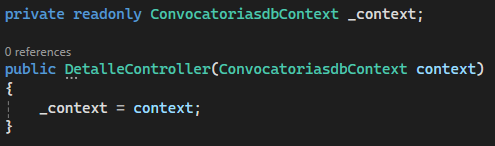
\includegraphics[width=0.7\linewidth]{DocumentacionTFG//img/InyeccionDependencias.PNG}
    \caption{Inyección de dependencias}
\end{figure}

\subsubsection{Patrón MVVM (Modelo-Modelo de Vista-Modelo)}

Este patrón aisla la vista del modelo y el modelo de la vista. La función principal del modelo de vista en este caso es proporcionar una representación de los datos que se adapte a la vista \cite{patronmvvm:latex}. Esto permite separar la lógica de presentación de la lógica de negocio y por lo tanto se evita que se realicen cambios importantes en el código del modelo.

En .NET este patrón se ha aplicado creando una serie de clases \textit{ViewModel} en las cuales solo se incluían los atributos que fuesen necesarios para una vista en concreto. De esta manera se evitan realizar cambios en el modelo de datos.

\begin{figure}[H]
    \centering
    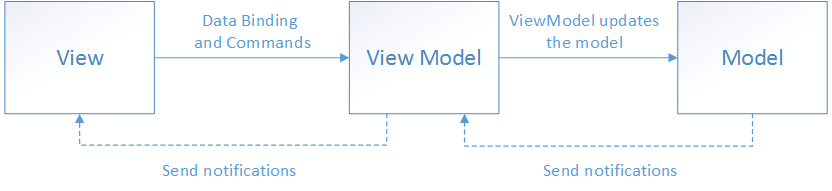
\includegraphics[width=0.9\linewidth]{DocumentacionTFG//img/PatronMVVM.png}
    \caption{Patrón MVVM}
\end{figure}

\subsubsection{Patrón Estrategia}
Este patrón se aplicó en el proceso de web \textit{scraping}, su principal propósito es permitir al objeto cliente elegir cual de las estrategias le conviene.

En el caso del proyecto, se dispone una serie de algoritmos de scraping en función de cada universidad. Estos algoritmos estarán cada uno en clases separadas pero todos ellos implementarán una interfaz común. Esto hace que según la universidad de la que se quiera hacer el \textit{scraping}, se selecciona su estrategia \cite{patronestrategia:latex}.

El patrón estrategia puede ser muy interesante de cara a futuro si se incluyen nuevas universidades en la aplicación dado que facilita enormemente las nuevas implementaciones y el testeo.
\begin{figure}[H]
    \centering
    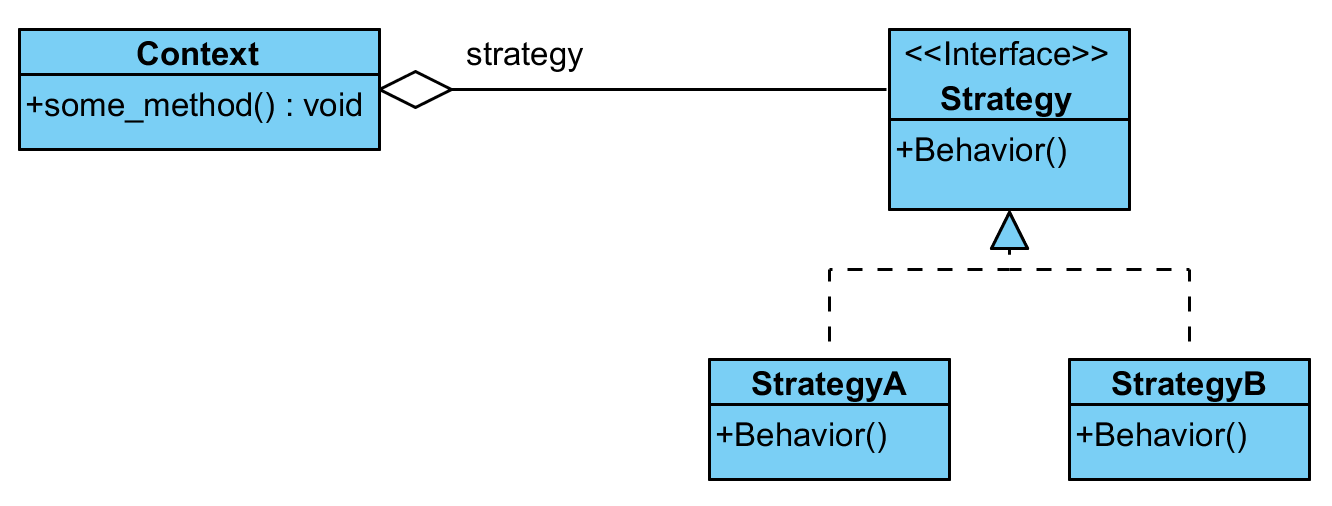
\includegraphics[width=0.7\linewidth]{DocumentacionTFG/img/PatronEstrategia.png}
    \caption{Patrón Estrategia}
\end{figure}

\subsection{Arquitectura general del sistema}
Para lograr el objetivo de desplegar la aplicación, se tuvo que diseñar una arquitectura en la que se utilizaron distintas herramientas para desplegar los diferentes componentes del sistema. En esta apartado se van a detallar cada una de las partes de la arquitectura del sistema tal y como se muestra gráficamente en \ref{img-diagrama-general}.

En primer lugar, mencionar que el sistema desarrollado tiene dos partes. Por un lado, tenemos la parte del web \textit{scraping} con Python con la que se recopilaban los datos y se actualizaba la base de datos. Por otro lado, tenemos la aplicación realizada con el \textit{framework} .NET Core MVC, esta aplicación obtiene los datos de la base de datos actualizada mediante \textit{web scraping} y los muestra en la web. Esta web es la que será utilizada por el usuario final.

Para el despliegue se ha desarrollado una arquitectura con tres componentes clave, las herramientas utilizadas se detallarán de manera más concreta en el capítulo 4 de la memoria. Aquí, se van a mencionar para un mejor entendimiento de la arquitectura.
\begin{itemize}
    \item \textbf{Servidor de Azure Database para MySQL:} En este servidor en la nube, se ha desplegado la base de datos MySQL. Esta decisión se ha tomado de esta manera debido a la facilidad que nos proporciona Azure para realizar despliegues sin realizar tareas de infraesctructura.
    \item \textbf{GitHub Action:} Esta herramienta es utilizada para la automatización de flujos de trabajo. En el sistema, se ha utilizado esta herramienta para crear una tarea programada que ejecutará el proyecto en Python y por lo tanto hará que la base de datos se actualice de manera periódica.
    \item \textbf{Azure App Services:} Este es un servicio basado en HTTP que permite hospedar aplicaciones web en la nube. En nuestro sistema, es el encargado de lanzar y alojar la aplicación desarrollada en .NET en la nube. Esto fue sencillo debido a que tanto Azure como .NET son propias de Microsoft por lo tanto el despliegue se pudo realizar con facilidad. Para que la información de la base de datos se mostrase correctamente en la web desplegada, se tuvieron que configurar las variables de entorno de este App Service e introducir la cadena de conexión de la base de datos desplegada en el servidor Azure Database. Este fue el último paso del montaje de la arquitectura del sistema y por lo tanto ya estaba la aplicación funcional disponible para utilizarse.
    \item \textbf{Usuario:} Es el encargado de interactuar con la aplicación. Para ello, accederá a la URL proporcionada por el servicio de Azure.  
\end{itemize}


\newpage
\begin{landscape}
\subsubsection{Diagrama arquitectura general del sistema}
\vspace{2cm}
\imagenapaisada{DiagramaGeneralArquitectura}{Diagrama arquitectura general del sistema.}\label{img-diagrama-general}   
\end{landscape}
\newpage


\section{Diseño de interfaces}
Dado que no había utilizado ninguna herramienta de \textit{mockup} recientemente y me parecía demasiado arcaico realizar diseños de interfaces a mano, decidí realizar los prototipos en sucio con PowerPoint. Esta decisión se tomó debido a la facilidad de uso que proporciona esa herramienta. 

Estos prototipos se fueron creando mediante la utilización de formas, contornos, fuentes, etc. A pesar de que la herramienta utilizada no es especifica para realizar los prototipos, el resultado fue satisfactorio.

\begin{figure}[H]
    \centering
    \includegraphics[width=0.8\linewidth]{DocumentacionTFG//img/MaestroDiseño.png}
    \caption{Diseño Ventana Maestra}
\end{figure}

\begin{figure}[H]
    \centering
    \includegraphics[width=0.8\linewidth]{DocumentacionTFG//img/DetalleDiseño.png}
    \caption{Diseño Ventana Detalle}
\end{figure}

\begin{figure}[H]
    \centering
    \includegraphics[width=0.8\linewidth]{DocumentacionTFG//img/DiseñoAdaptativo.png}
    \caption{Diseño Adaptativo}
\end{figure}

Estos prototipos surgieron como idea inicial. Las interfaces reales se han ido modificando a medida que se iban programando para que sean mas atractivas para el usuario.

\apendice{Documentación técnica de programación}

\section{Introducción}

\section{Estructura de directorios}

\section{Manual del programador}

\section{Compilación, instalación y ejecución del proyecto}

\section{Pruebas del sistema}

\apendice{Documentación de usuario}

\section{Introducción}

\section{Requisitos de usuarios}

\section{Instalación}

\section{Manual del usuario}



\apendice{Anexo de sostenibilización curricular}

\section{Introducción}
Este anexo incluirá una reflexión personal del alumnado sobre los aspectos de la sostenibilidad que se abordan en el trabajo.
Se pueden incluir tantas subsecciones como sean necesarias con la intención de explicar las competencias de sostenibilidad adquiridas durante el alumnado y aplicadas al Trabajo de Fin de Grado.

Más información en el documento de la CRUE \url{https://www.crue.org/wp-content/uploads/2020/02/Directrices_Sosteniblidad_Crue2012.pdf}.

Este anexo tendrá una extensión comprendida entre 600 y 800 palabras.



\bibliographystyle{plain}
\bibliography{bibliografiaAnexos}

\end{document}
